\section{Beta Distribution}

\subsection{Standard Beta Distribution}

The pdf of the Beta distribution in the standard basis is

\begin{equation}
	f(x, \alpha, \beta) = \frac{x^{(\alpha - 1)} \cdot (1-x)^{(\beta-1)}}{B(\alpha, \beta)} \\
\end{equation}

where $B(\alpha, \beta) = \frac{\Gamma(\alpha)\Gamma(\beta)}{\Gamma(\alpha + \beta)}$ and $\Gamma(x)$ is the Gamma function. This can be written as 

\begin{align}
	f(x, \alpha, \beta) &=  \exp\left[(\alpha-1) \log(x) + (\beta-1)\log(1-x) - \log(B(\alpha,\beta)))\right]\\
	&= \frac{1}{x(1-x)}\exp\left[\alpha\log(x) + \beta\log(1-x) - \log(B(\alpha,\beta)))\right]
\end{align}

With $h(x) = \frac{1}{x(1-x)}, T=(\log(x), \log(1-x), \eta = (\alpha, \beta)$ and $A(\alpha, \beta) = \log(B(\alpha,\beta)))$. 


\subsubsection{Laplace approximation of the standard Beta distribution}

To get the Laplace approximation we need the mode and Hessian. To get the mode we use the first derivative of the log-pdf and set it to zero. To get the Covariance we use the Hessian at the mode, multiply it with -1 and invert it. 

\begin{align*}
\text{log-pdf: } &\log\left( \frac{x^{(\alpha - 1)} \cdot (1-x)^{(\beta-1)}}{B(\alpha, \beta)} \right) \\
&= (\alpha-1) \log(x) + (\beta-1)\log(1-x) - \log(B(\alpha,\beta)))\\
\text{1st derivative: }& \frac{(\alpha-1)}{x} - \frac{(\beta-1)}{1-x}  \\
\text{mode: }& \frac{(\alpha-1)}{x} - \frac{(\beta-1)}{1-x}  = 0 \Leftrightarrow x = \frac{\alpha-1}{\alpha + \beta - 2} \\
\text{2nd derivative: }& \frac{\alpha -1}{x^2} + \frac{\beta - 1}{(1 - x)^2} \\
\text{insert mode: }& \frac{\alpha -1}{\frac{\alpha-1}{\alpha + \beta - 2}^2} + \frac{\beta - 1}{(1 - \frac{\alpha-1}{\alpha + \beta - 2})^2} = \frac{(\alpha + \beta - 2)^3}{(\alpha-1)(\beta-1)}\\
\text{invert: }& \frac{(\alpha -1)(\beta-1)}{(\alpha + \beta - 2)^3}
\end{align*}

The Beta distribution in standard basis is therefore approximated by $N(\mu = \frac{\alpha-1}{\alpha + \beta - 2}, \sigma^2 = \frac{(\alpha -1)(\beta-1)}{(\alpha + \beta - 2)^3})$.

\subsection{Logit-Transform of the Beta distribution}

We transform the Beta distribution using $g(x) = \log(\frac{x}{1-x})$. Therefore $g^{-1}(x) = \sigma(x) = \frac{1}{1+ \exp(-x)}$. This yields the following pdf

\begin{align}
	f_t(x, \alpha, \beta) &= \frac{1}{\sigma(x)(1-\sigma(x))}\exp\left[\alpha\log(\sigma(x))) + \beta\log(1-\sigma(x)) - \log(B(\alpha,\beta)))\right] \cdot (\sigma(x)(1-\sigma(x)) \\
	&= \exp\left[\alpha\log(x) + \beta\log(1-x) - \log(B(\alpha,\beta)))\right] \nonumber
	\label{eq:beta_logit_trans_pdf}
\end{align}

Which has $h(x) = 1, T=(\log(\sigma(x)), \log(1-\sigma(x)), \eta = (\alpha, \beta)$ and $A(\alpha, \beta) = \log(B(\alpha, \beta))$.

\subsubsection{Laplace approximation of the logit transformed Beta distribution}

mode and variance of log pdf blablabla

\begin{align*}
\text{log-pdf: } &\log\left( \frac{\sigma(x)^{\alpha} \cdot (1 - \sigma(x)^{\beta})}{B(\alpha, \beta)} \right) \\
&= \alpha \log(\sigma(x)) + \beta \log(1 - \sigma(x)) - \log(B(\alpha, \beta))\\
\text{1st derivative: }&  \alpha (1 - \sigma(x)) - \beta \sigma(x)\\
\text{mode: }& \alpha (1 - \sigma(x)) - \beta \sigma(x) = 0 \Leftrightarrow x = -\log(\frac{\beta}{\alpha}) \\
\text{2nd derivative: }& (\alpha + \beta)\sigma(x)(1 - \sigma(x))  \\
\text{insert mode: }& (\alpha + \beta)\sigma(-\log(\frac{\beta}{\alpha}))(1 - \sigma(-\log(\frac{\beta}{\alpha}))) = \frac{\alpha\beta}{\alpha + \beta}  \\
\text{invert: }& \frac{\alpha + \beta}{\alpha \beta}
\end{align*}


The LPA is therefore $\mathcal{N}(\mu=-\log(\frac{\beta}{\alpha}), \sigma^2 = \frac{\alpha + \beta}{\alpha \beta})$.

\subsubsection{The Bridge for the logit transformation}


\begin{figure}[!htb]
	\centering
	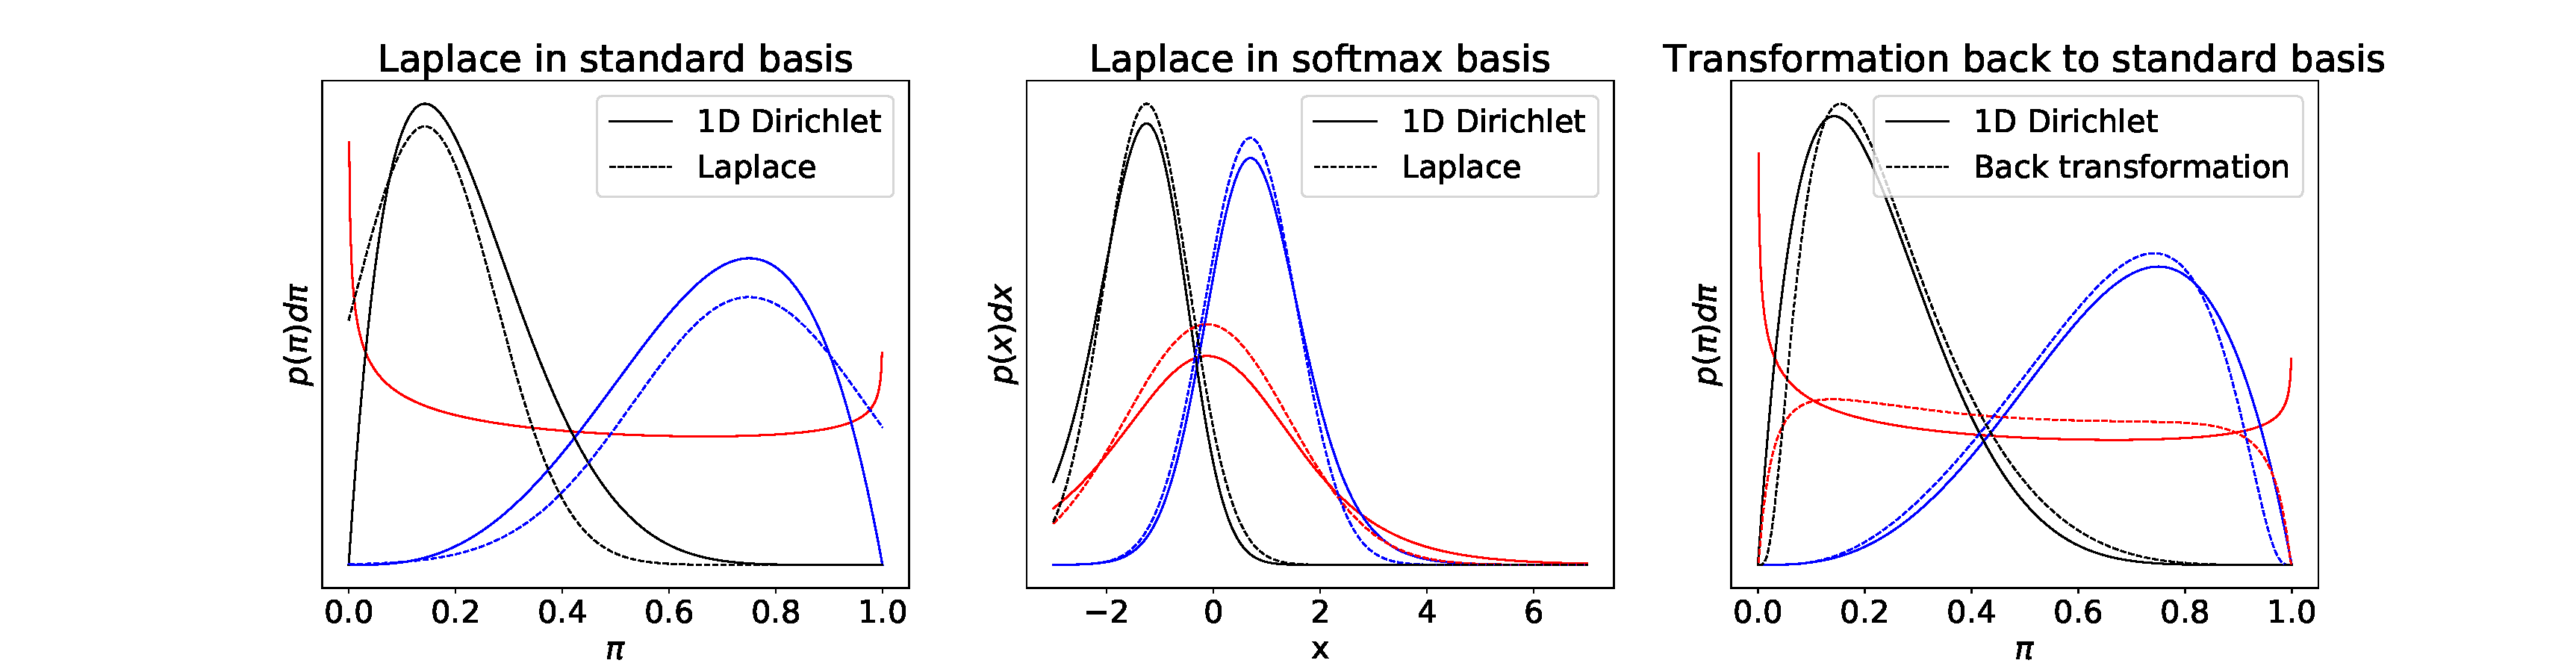
\includegraphics[width=\textwidth]{figures/beta_playground.pdf}
	\caption{beta comparison}
	\label{fig:beta_comparison}
\end{figure}